

\section{Implementation}
Most of the theorie behind RS and the methodology it depends on have already been introduced.
The implementation of a RS will be described in the following.
The examples will be written in a programming language called Python.
There is also some SQL code and some UML- and EER-diagrams in order to visualize the concept.

\subsection{Content based RS in-depth}
\label{sec:implementation-contentbased}
The general framework for a content-based RS is shown in figure~\ref{fig:framework-contentbasedrs}.
There are three main components a content-based RS needs.
\begin{itemize}
    \item \textbf{Content Analyzer}\\
        Since all items the RS has to work with can potentially be unstructured, a pre-process is necessary to filter relevant information.
        This will be mainly done by techniques of IR.
        The Content Analyzer aims to bring all items in a from that can be used by its successional components.
        \citep[p.~75-77]{lops:2011}
    \item \textbf{Profile Learner}\\
        When the items are in a suitable form, the Profile Learner can construct a user profile.
        In case of Rocchio's algorithm this includes to distinguish all relevant items from non-relevant.
        With the items and the users preferences the Profile Learner can build the user profile.
        In case of Rocchio, the user profile is a vector representing his attitude towards the different attributes a item may have.
        \citep[p.~75-77]{lops:2011}
    \item \textbf{Filtering Component}\\
        For each user profile the Filtering Component can find items that may match the users preferences.
        Depending on the method implemented the result can be a binary or continuous relevance judgment.
        The continuous relevance judgement is a list of ranked items.
        \citep[p.~75-77]{lops:2011}
        The RS implemented for this thesis uses the k-nearest-neighbours algorithm.
        This results in a list of ranked items where the best-ranked items will be suggested to the user.
\end{itemize}




\begin{figure}[h]
    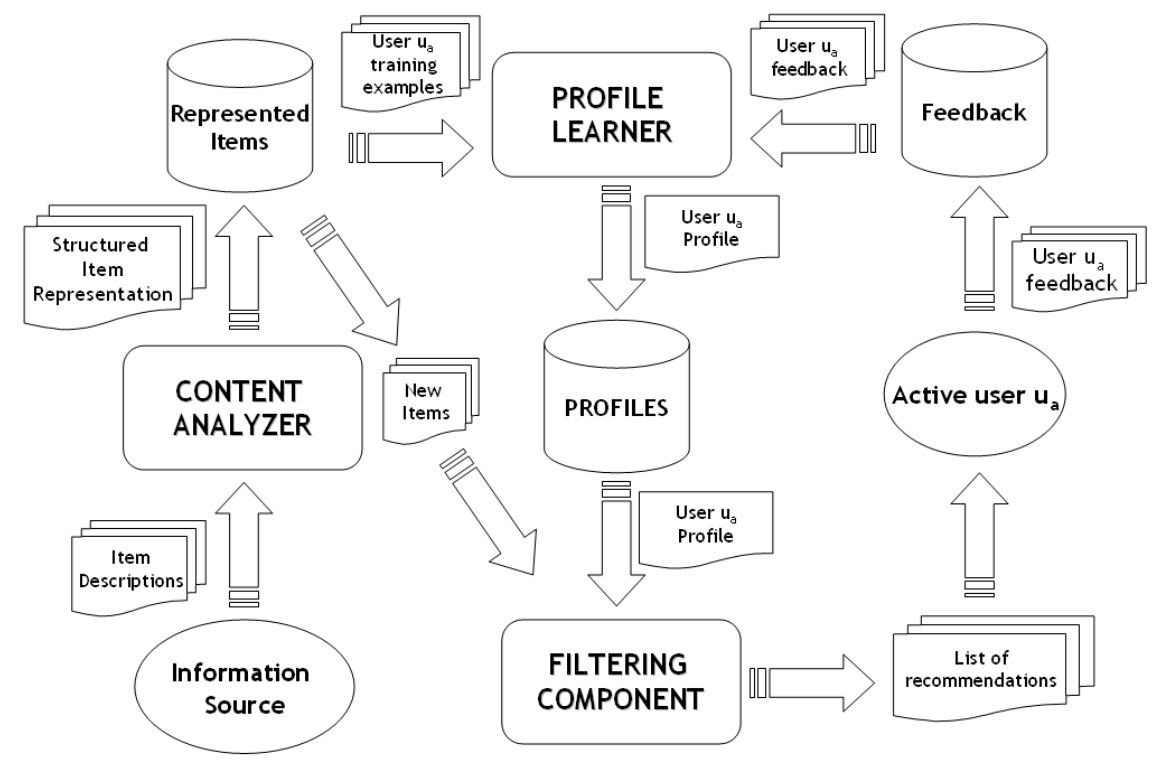
\includegraphics[scale=0.3]{inc/rocchio/HighlevelContentBased}
    \caption{High level description of a content-based RS.\citep[p.~76]{lops:2011}}
    \label{fig:framework-contentbasedrs}
\end{figure}

\subsection{Content Analyzer}
%{Building the vectors}
%{Storage within the database}


\subsection{Profile Learner}
%{Rocchio algorithm}
%{Relevance feedback}

\subsection{Filtering Component}


%%%%%%%%%%%%%%%%%%%%%%%%%%
%k nearest neighbours
% manning 297, 290 (euclidean distance)
%%%%%%%%%%%%%%%%%%%%%%%%%%

\subsection{Onlineshop}
... dunno

\subsection{Testing}
wie sind die Empfehlungen des algorithmus
